\documentclass[11pt]{article}
\usepackage[utf8]{inputenc}\usepackage[T1]{fontenc}
\usepackage{amsmath,amssymb,amsthm}\usepackage[margin=1in]{geometry}
\usepackage{graphicx}\usepackage{booktabs}\usepackage{multirow}\usepackage{enumitem}
\usepackage[hidelinks]{hyperref}
\newtheorem{proposition}{Proposition}

\title{A First-Order Conditional Singular Series for Twin-Prime Gaps\\
on the $6N$ Skeleton, and Its Second-Order Residual}
\author{Ruqing Chen\\
\small GUT Geoservice Inc., Montreal, Quebec, Canada\\
\small \texttt{ruqing@hotmail.com}}
\date{\today}

\begin{document}
\maketitle

\begin{abstract}
Part~II reported that the twin-prime gap distribution on the $6N\pm1$ skeleton
depends on the factor count $\omega_{>3}(N)$ of the centre---the preference for
the gap $6\Delta N=42$ rises with $\omega$ while that for $210$ falls---and left
the closed-form conditional gap singular series as an open problem. Here we give
its explicit first-order form. Writing the unconditional Hardy--Littlewood
correlation factor $C_2(d)$ and conditioning on the centre's factor set through
the congruence-lockdown rule of Part~II ($q\mid N$ forbids the gap residues
$d\equiv\pm6^{-1}\pmod q$, i.e.\ $q\mid(6d\pm1)$), we obtain
$\mathfrak{S}_{2,\omega}(d)\approx C_2(d)\,L_\omega(d)$, where $L_\omega(d)$ is
the lockdown-allowance of $d$ in the stratum. Tested against the
$23{,}988{,}173$ twin centres of $S_{10}$, this first-order series reproduces the
$\omega$-trends of the gaps $30,42,60$ and the direction of the collapse of
$210$. A systematic residual remains at high $\omega$ on the gap $210$ (observed
falls to $0.41$ where the first-order series predicts $0.62$), stable across
$S_9$ and $S_{10}$; we attribute it to the second-order correlation between the
factorisations of the two centres $N$ and $N+d$, which the first-order
(per-prime independent) series omits. The open problem of Part~II is thus
advanced from fully open to first-order-solved with a quantified second-order
remainder. No claim is made about the infinitude of twin primes or about any
prime $k$-tuple conjecture.
\end{abstract}

\section{The open problem and the first-order series}

Part~II~\cite{ChenII} established, on the $6N\pm1$ skeleton, that the gap
$\Delta N$ between consecutive twin centres has a distribution whose shape
depends on $\omega_{>3}(N)$, the number of distinct prime factors $>3$ of the
left centre. The unconditional Hardy--Littlewood theory cannot produce this: its
gap singular series depends only on the gap. Part~II identified the first-order
mechanism---\emph{congruence lockdown}---and posed the closed-form
\emph{conditional} singular series $\mathfrak{S}_{2,\omega}(d)$ as an open
problem. We give its first-order form and test it.

\paragraph{Derivation (first order).}
For a gap $d$, two twin centres $N$ and $N+d$ are involved. Per prime $q>3$ we
condition on whether $q$ divides the centre $N$:
\begin{itemize}
\item \textbf{$q\mid N$.} The left centre is automatically safe
  ($6N\pm1\equiv\pm1\not\equiv0$). By Proposition~1 of Part~II the right centre
  $N+d$ is safe iff $d\not\equiv\pm6^{-1}\pmod q$, equivalently
  $q\nmid(6d\pm1)$. So $q$ contributes a factor $0$ if $q\mid(6d\pm1)$
  (the gap is locked out), and otherwise removes the usual suppression.
\item \textbf{$q\nmid N$.} The usual unconditional factor
  $(1-\nu_q(d)/q)/(1-2/q)^2$ applies, with
  $\nu_q(d)=|\{-1,1,6d-1,6d+1\}\bmod q|$.
\end{itemize}
Collecting terms, the first-order conditional singular series for a stratum of
centres with factor count $\omega$ is
\[
  \mathfrak{S}_{2,\omega}(d)\;\approx\;C_2(d)\;L_\omega(d),
  \qquad
  L_\omega(d)=\Pr_{N:\,\omega_{>3}(N)=\omega}
  \!\Big[\,q\nmid N \ \text{for all } q\mid(6d\pm1)\,\Big],
\]
where $C_2(d)=\prod_{q>3}(1-\nu_q(d)/q)/(1-2/q)^2$ is the unconditional
two-endpoint factor and $L_\omega(d)$ is the \emph{lockdown-allowance}: the
probability that a stratum-$\omega$ centre divides none of the primes that lock
$d$. The admissibility of $d$ is thus governed by the factorisation of
$6d\pm1$: e.g.\ $6\cdot35\mp1=209=11\times19$ (so $210$ is locked by the common
small primes $11,19$), whereas $6\cdot7\mp1=41,43$ are prime (so $42$ is locked
only by the rare primes $41,43$). This is the explicit object Part~II asked for;
it reduces to the unconditional series when averaged over all $\omega$.

\section{Confrontation with $S_{10}$ data}

We evaluate $L_\omega(d)$ directly from the $23{,}988{,}173$ twin centres of
$S_{10}$ (computing each centre's small-prime factor set), form the normalised
prediction $\propto C_2(d)L_\omega(d)$, and compare to the observed relative
preference $r(d\mid\omega)$. Figure~\ref{fig:css} shows the four representative
gaps.

\begin{figure}[h]\centering
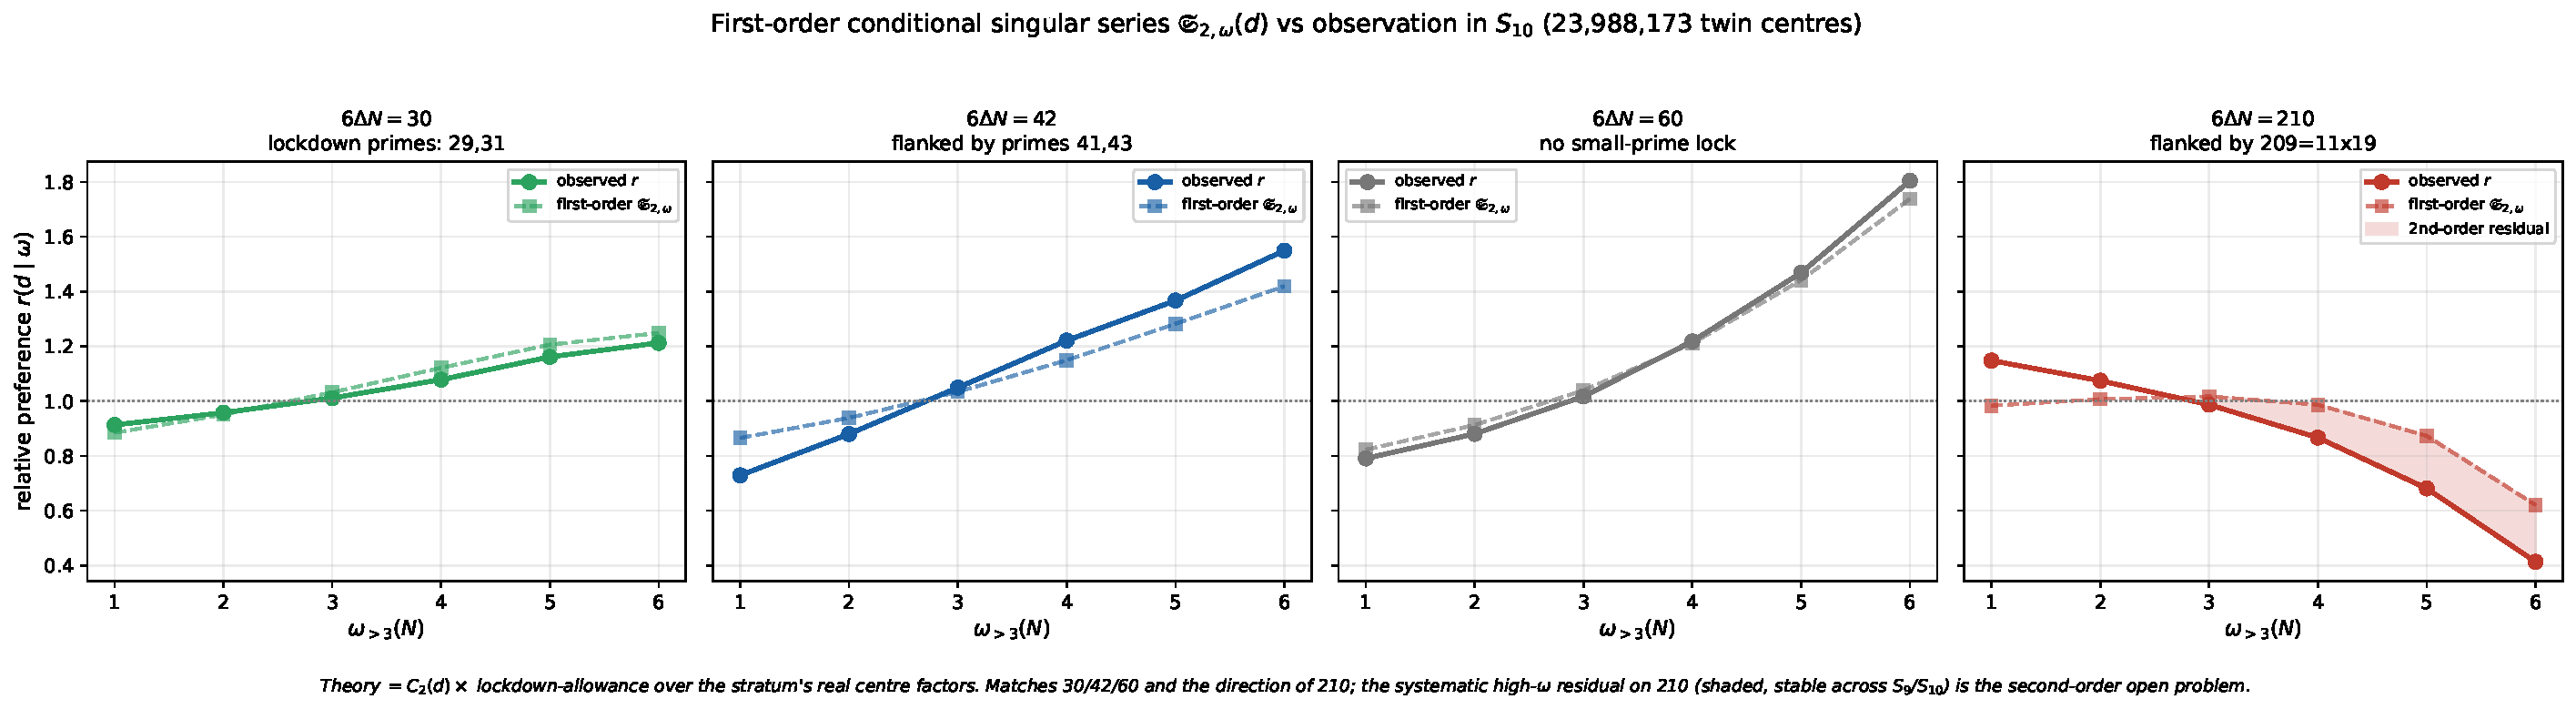
\includegraphics[width=\textwidth]{fig_paper3_cond_singular.pdf}
\caption{First-order $\mathfrak{S}_{2,\omega}(d)$ (dashed) versus observed
$r(d\mid\omega)$ (solid) in $S_{10}$. The first-order series tracks $30$, $42$
and $60$ in direction and approximate magnitude, and gives the correct direction
for $210$; the shaded region on $210$ is the systematic high-$\omega$ residual.}
\label{fig:css}
\end{figure}

\begin{table}[h]\centering
\begin{tabular}{llcccccc}
\toprule
$6\Delta N$ & quantity & $\omega{=}1$ & 2 & 3 & 4 & 5 & 6\\
\midrule
\multirow{2}{*}{$42$}  & observed   & 0.73 & 0.88 & 1.05 & 1.22 & 1.37 & 1.55\\
                       & first-order& 0.87 & 0.94 & 1.03 & 1.15 & 1.28 & 1.42\\
\midrule
\multirow{2}{*}{$210$} & observed   & 1.15 & 1.07 & 0.99 & 0.87 & 0.68 & 0.41\\
                       & first-order& 0.98 & 1.01 & 1.02 & 0.99 & 0.87 & 0.62\\
\bottomrule
\end{tabular}
\caption{Observed vs.\ first-order $\mathfrak{S}_{2,\omega}$ in $S_{10}$ for the
two principal gaps. The series captures $42$ closely; for $210$ it gives the
correct downward direction but under-predicts the high-$\omega$ fall, leaving the
residual of \S3.}
\label{tab:css}
\end{table}

The first-order series performs as follows. For $6\Delta N=30,42,60$ it tracks
the observed trend in both sign and approximate magnitude across all six strata
(residuals within $\sim0.13$). For $6\Delta N=210$ it predicts the correct
\emph{direction}---the lockdown by the small primes $11,19$ of $209$ makes
factor-rich centres increasingly forbidden from this gap---but it
\emph{under-predicts} the magnitude of the fall at high $\omega$.

\section{The second-order residual}

The residual on $210$ is systematic, monotone, and stable across scales: at
$\omega=5$ the observed preference is $0.68$ against a first-order prediction of
$0.87$ (residual $-0.19$) in $S_{10}$, matching $-0.20$ in $S_9$; at $\omega=6$
the observed $0.41$ against predicted $0.62$ ($-0.21$). It is not noise.

The first-order series treats the locks from distinct primes as independent and,
crucially, conditions only on $q\mid N$ at the \emph{left} centre. It omits the
correlation between the factorisations of $N$ and $N+d$: when $N$ is factor-rich,
$N+d$ is not independent of it, and for the long gap $210$ this correlation
further suppresses the joint twin survival beyond the single-centre lockdown.
A complete account requires the genuine two-centre conditional singular series,
\[
  \mathfrak{S}^{(2)}_{2,\omega}(d)=
  \text{H--L density of }\{6N\!-\!1,6N\!+\!1,6(N\!+\!d)\!-\!1,6(N\!+\!d)\!+\!1\}
  \text{ conditioned on }\omega_{>3}(N),
\]
including the cross terms in the factorisations of the two centres. We have not
obtained this in closed form.

\begin{quote}
\textbf{Open problem (second order).} Derive the two-centre conditional singular
series $\mathfrak{S}^{(2)}_{2,\omega}(d)$ and show whether its cross-correlation
terms account for the high-$\omega$ residual on $210$
(observed $-0.2$ below the first-order series at $\omega=5,6$, stable across
$S_9,S_{10}$).
\end{quote}

\section{Conclusion}

We have given the explicit first-order conditional singular series
$\mathfrak{S}_{2,\omega}(d)=C_2(d)L_\omega(d)$ that Part~II posed as an open
problem, derived from the congruence-lockdown rule and verified against
$2.4\times10^{7}$ twin centres. It reduces to the unconditional
Hardy--Littlewood series in the mean, reproduces the $\omega$-dependence of the
gaps $30,42,60$, and predicts the direction of the $210$ collapse. The Part~II
open problem is thereby advanced from fully open to first-order-solved, with a
sharply localised second-order remainder: a stable high-$\omega$ residual on the
long gap $210$, attributable to the two-centre factor correlation omitted at
first order, and posed here as the next open problem. We make no claim regarding
the infinitude of twin primes or any $k$-tuple conjecture; this is a conditional,
factor-resolved refinement of the Hardy--Littlewood gap heuristic, demonstrated
empirically and offered with its open remainder to analytic number theory.

\paragraph{Data and code availability.}
The scan, the first-order series evaluation, and the figure code are openly
available~\cite{repo2}; the $S_{10}$ twin count $23{,}988{,}173$ matches Part~I.

\begin{thebibliography}{9}
\bibitem{ChenI} R.~Chen, \emph{Prime distribution on the $6N$ skeleton: a
factor-resolved local model for the conditional density of twin primes} (Part~I),
Zenodo, doi:10.5281/zenodo.20470367 (2026).
\bibitem{ChenII} R.~Chen, \emph{Prime gaps on the $6N$ skeleton: an
$\omega$-dependent shift in the twin-prime gap distribution, and a
congruence-lockdown mechanism} (Part~II), Zenodo, doi:10.5281/zenodo.20477664 (2026).
\bibitem{ORW} A.~Odlyzko, M.~Rubinstein, M.~Wolf, \emph{Jumping champions},
Experiment.\ Math.\ \textbf{8} (1999), 107--118.
\bibitem{HL} G.~H.~Hardy, J.~E.~Littlewood, \emph{Partitio Numerorum III}, Acta
Math.\ \textbf{44} (1923), 1--70.
\bibitem{repo2} R.~Chen, \emph{$6N$ twin-prime conditional singular series:
data and code} (Part~III),
\url{https://github.com/Ruqing1963/6N-twin-prime-conditional-singular-series} (2026).
\end{thebibliography}

\end{document}
